\documentclass{sig-alternate}
\usepackage{mathtools}
\usepackage{color}
% For displaying Scala source code
\usepackage{listings}
\lstdefinelanguage{Scala}{
  morekeywords={abstract,case,catch,class,def,%
    do,else,extends,false,final,finally,%
    for,if,implicit,import,match,mixin,%
    new,null,object,override,package,%
    private,protected,requires,return,sealed,%
    super,this,throw,trait,true,try,%
    type,val,var,while,with,yield},
  otherkeywords={=>,<-,<\%,<:,>:,\#,@},
  sensitive=true,
  morecomment=[l]{//},
  morecomment=[n]{/*}{*/},
  morestring=[b]",
  morestring=[b]',
  morestring=[b]"""
}
\lstset{language=Scala, basicstyle={\small\ttfamily}}

\usepackage{blindtext,tikz}
\usetikzlibrary{calc}


%\usepackage{graphicx,eso-pic,xcolor}
%\makeatletter
%\AddToShipoutPicture{%
%\setlength{\@tempdimb}{.5\paperwidth}%
%\setlength{\@tempdimc}{.5\paperheight}%
%\setlength{\unitlength}{1pt}%
%\put(\strip@pt\@tempdimb,\strip@pt\@tempdimc){%
 %   \makebox(-500,200){\rotatebox{90}{\textcolor[gray]{0.70}%
 %      {\Large \textsf{Draft of \today}}}}
 % }%
%}
%\makeatother


% For commenting
\newcommand{\comment}[1]{{\small \color{red} {#1}} \normalcolor}
% Use this line for leaving out comments
%\newcommand{\comment}[1]{}

% Notation commands (change all by changing here)
% Defina a capital Rho
\newcommand{\Rho}{\mathrm{P}}
% Concept relation
\newcommand{\rn}[1]{\rho_{#1}}
% Concept L1 norm
\newcommand{\rns}[1]{|\rn{#1}|_1}
% Concept relation threshold
\newcommand{\mrn}[1]{\tau_{#1}}
% Discarded concept relation sum
\newcommand{\drns}[1]{|\check{\rho}_{#1}|_1}
% Kept concept relation sum
\newcommand{\krns}[1]{|\hat{\rho}_{#1}|_1}
% Concept relation vector
\newcommand{\rv}{\Rho}

% Concept similarity
\newcommand{\sy}[1]{\sigma_{#1}}
% Approximate concept similarity
\newcommand{\asy}[1]{\tilde{\sigma}_{#1}}
% L1 norm of difference
\newcommand{\nm}[1]{L_1(#1)}
\newcommand{\dnm}[2]{|\rn{#1}-\rn{#2}|_1}
% Approximate L_1 norm
\newcommand{\anm}[1]{\tilde{L}_1(#1)}

\hyphenation{adap-ta-tion dis-t-ri-bu-ted de-tec-tion net-wo-rk cha-n-ges}

\begin{document}

\title{Knowing a concept by the company it keeps:\\Scalable concept discovery through commutability}

\numberofauthors{3}
\author{
\alignauthor
Olof G\"{o}rnerup\\ %\titlenote{}\\
       \affaddr{Swedish Institute of}\\
       \affaddr{Computer Science (SICS)}\\
       \affaddr{SE-164 29 Kista, Sweden}\\
       \email{olof@sics.se}
\alignauthor
Daniel Gillblad\\ %\titlenote{}\\
       \affaddr{Swedish Institute of}\\
       \affaddr{Computer Science (SICS)}\\
       \affaddr{SE-164 29 Kista, Sweden}\\
       \email{dgi@sics.se}
\alignauthor
Theodore Vasiloudis\\ %\titlenote{}\\
       \affaddr{Swedish Institute of}\\
       \affaddr{Computer Science (SICS)}\\
       \affaddr{SE-164 29 Kista, Sweden}\\
       \email{tvas@sics.se}
%\and  % use '\and' if you need 'another row' of author names
}


%\toappear{}

\maketitle

\tikz[overlay,remember picture]
{
     \node at ($(current page.west)+(1, 15)$) [rotate=90] {\huge\textcolor{gray}{Preprint 20 Feb.\ 2015}};
}

\begin{abstract}
\begin{sloppypar}
Discovering higher-order concepts, or representations of abstract ideas and notions, directly from large data sets has
a large potential both for understanding data and generating processes, and for building efficient representations. Here, we
rely on a general and commonly valid principle of similarity among objects based on notions of context and
commutability for concept discovery. We develop a scalable, data-driven, and graph-based approach for discovering
similar objects, where similarity is expressed in terms of their respective context. We show that the
error in approximations of this similarity can be bound and used to achieve fast calculations, and that groups of
similar objects in the resulting similarity graph can be used to represent higher-order concepts. These principles and
methods are applicable in a broad range of domains, but will here be demonstrated for three distinct types of objects:
words, artists and codons, with data sets ranging from small to very large both in terms of examples and number
of objects.
\end{sloppypar}
\end{abstract}

\category{I.2.6}{Artificial Intelligence}{Analogies}
\category{I.5.3}{Clustering}{Algorithms, Similarity measures}
\category{H.2.8}{Database Management}{Database Applications -- Data Mining}

\terms{Algorithms, Design, Experimentation}

\keywords{Concept discovery, graph algorithms, community detection, clustering}

\section{Introduction}

As stated by Firth \cite{Firth57} and further popularized in the computational linguistics community by Church and
Hanks \cite{Church90}, ``You shall know a word by the company it keeps''. Departing from this principle, there have
been substantial efforts in for example machine learning to infer semantic and syntactic meaning from words through their effective
usage in text and speech. Although the same principle has been applied in other domains, such as recommendation
systems, generalizing the notion of characterizing concepts through their contexts into a broader fundamental principle
for knowledge discovery is so far largely unexplored.

Extending Firth's line of thought we argue that the effective semantics of any concept are given by the context in which
it occurs, or in other words, by how it is related (or correlated) to all other concepts. The \emph{similarity} between
two concepts may therefore be formulated in terms of their contexts, or how similar their relations to all other
concepts are.
In essence, we focus on the commutability (or exchangeability) of concepts.
A benefit of this is that we can omit the specific functionality or underlying workings of concepts, but
only observe and consider their context patterns. This is highly attractive from a data-driven machine learning
perspective since it requires few assumptions.

With this as a starting point, we propose a graph-based method for discovering higher order concepts from large data
sets. A \emph{concept} is intentionally left vague since it can be many different things, such as tokens in a text,
music tracks in a playlist, people in a social network or states in a stochastic process. We narrow down the scope
slightly by only considering concepts that exhibit pairwise relations, e.g.\ in terms of spatial, temporal or social
correlations, which allows us to represent a collection of concepts and their inter-dependencies as a graph. Our
approach can then be summarized as
\begin{enumerate}
\item Create a \emph{correlation graph} that describes the pairwise correlations between all concepts. A correlation may here be any relationship measure such as
the frequency of co-occurrence, a correlation measure such as mutual information, a weighted edge in a graph, a
transition probability in a stochastic process.
\item Transform the correlation graph to a \emph{similarity graph} by comparing the set of correlation of each concept
to the set of correlations of all other concepts -- the more similar set of correlations, the higher the weighted edge in the
similarity graph. Here, we base our similarity measure on the $L_1$-norm.
\item Find clusters in terms of strongly connected communities in the similarity graph. These clusters contain concepts
that play a similar role in data (i.e. they are commutable), and each cluster is considered to represent a higher-order
concept.
\end{enumerate} As we are considering an ``all-to-all" similarity problem when deriving the similarity graph, without
using any form of intermediate representation of contexts, this derivation is computationally challenging. To manage
this, we devise an approach to approximate the calculation while keeping the error low and controllable.

There are mainly two advantages of the direct similarity calculation compared to other (e.g. vector- and neural
network-based) approaches: First, the approach is interpretable and transparent. We can for example calculate
well-understood notions of similarity and error. Second, it allows us to be highly agnostic in terms of the correlation
measures, making it directly applicable in a large number of domains as well as potentially applicable
in mixed-data scenarios where several different correlation measures must be employed.

\begin{sloppypar} Finally, representing all objects and their correlations in graphs allow us to capture higher-scale
structures among objects, such ambiguity, concept hierarchies, and object ontologies, both in terms of dependencies and
similarities, in a straightforward manner.
\end{sloppypar}

\section{Related work}

Our work can be viewed as a way to determine and group semantic similarity between concepts, as defined in Section
\ref{sec:preliminaries}. A comprehensive survey of the field of semantic measures can found in
\cite{harispe2013semantic}, where the authors classify measures as distributional, knowledge-based, and hybrid.
In short, distributional measures make use of statistical analysis of unstructured data to derive
similarities, while knowledge-based measures make use of knowledge representations such as ontologies or lexical databases
and as such require a more structured input.

\begin{sloppypar}
Within language technology, distributional analysis -- where similarities between linguistic items are characterized by
their relative distributional properties in the data -- has become a fundamental approach \cite{Harris-1970}. We use
similar assumptions as a starting point, and when applied to text, the approach can be seen as transforming a graph
over syntagmatic similarities to one describing paradigmatic similarities \cite{Sahlgren-2006}, in which higher order
concepts are discovered through clustering. A large number of methods to find semantic similarities have been
developed, from different types of high-dimensional vector representations such as latent semantic analysis
\cite{Landauer-1998} and random indexing \cite{kanerva:hyperdimensional} to Kolmogorov complexity-based measures
\cite{Cilibrasi-2007} and neural network-based solutions such as word2vec \cite{Mikolov-2013}. While we use a
completely graph-based approach that is more domain agnostic and which essentially performs no dimensionality
reduction, several of these methods could be used to produce the equivalent of the similarity graph in which we perform
clustering to find higher order concepts.
\end{sloppypar}

%TODO(tvas): Apart from similarity calculation, the creation of higher order concepts is related to the problem of ontology learning.

Another approach for calculating similarities between linguistic items and creating higher order concepts is using
lexical databases such as WordNet \cite{miller1995wordnet}. While this approach has been used extensively
 (see surveys \cite{budanitsky2006evaluating}, \cite{lin2008survey}), its obvious disadvantage is
the need for the creation and maintenance of the database by experts. Jiang et al. \cite{jiang2011ontology} proposed a
method of automatically enhancing the WordNet ontologies by merging Wikipedia entities into WordNet, easing the
maintenance task, and proposed a learning approach that produces a set of concepts that semantically describe a
document collection.

%TODO(tvas): Include google similarity distance here as extra ref? Can also include Schedl paper for music co-oc then.
%\comment{Where does Google sim. distance belong?}
%In \cite{cilibrasi2007google} Cilibrasi et al. define the Google similarity distance as a way to measure the similarity
%between concepts.

Halawi et al. \cite{Halawi12} proposed an alternative approach which bridges
the statistical techniques and lexical database approaches by ``constraining the learning process with word pairs that
are known to be related''. The authors use a latent factor method to create low-dimensional
representations of words, but also impose regularization constraints in the learning
process for pairs of concepts that are known to be related, according to WordNet synonyms.
We effectively also limit the calculations of similarity values to pairs
of words that are related. However, our approach does not require an external lexical database, as the constraints
emerge from the correlation structure inherent in the data.

As a special case, our approach can also function as a hybrid method, since it is possible to use with a structured input
such as a correlation graph, but at the same time we provide intuitive ways to create the input correlation graph from
unstructured data, thereby making the method more general.

Although related approaches are recognized, concept discovery through commutability has
not quite established itself as a standard practice for knowledge discovery. We therefore hope that the general approach and scalable
solutions presented here can contribute to a more general use.

\section{Background}

\subsection{Preliminaries}
\label{sec:preliminaries}

Let $C = \{i\}_{i=1}^n$ be a set of \emph{concepts}, where each concept has a correlation, $\rn{i,j}$, to
each other concept. This relation can be expressed in terms of real values, probabilities, booleans or something
else, that, for instance, represent a correlation measure, binary or weighted neighbourhood relation in a graph,
co-occurrence probabilities in a corpus, or transition probabilities in a Markov chain.

The \emph{context} of a concept $i$ is considered to be its vector of relations to every other concept, $\rn{i} =
(\rn{i,j})_{j=1}^n$. Under the key assumption that a concept is characterized by its context, we can formulate the
similarity between two concepts $i$ and $j$, denoted $\sy{i,j}$, in terms of a similarity measure between their
respective contexts.
Here we define $\sy{i,j}$ to be one minus the relative $L_1$-norm of the difference between $\rn{i}$ and $\rn{j}$:
%Here we define $\sy{i,j}$ to be the inverse of the relative $L_1$-norm of the difference between $\rn{i}$ and $\rn{j}$:
\begin{equation}\label{eq:sim}
\sy{i,j} = 1 - \frac{\dnm{i}{j}}{\rns{i} + \rns{j}},
%\sy{i,j} = \frac{\rns{i} + \rns{j}}{\dnm{i}{j}},
%\sy{i,j} = \frac{\rns{i} + \rns{j}}{\nm{i,j}},
\end{equation}
where
\begin{equation}\label{eq:totrel}
\rns{i} = \sum_{k \in C} | \rn{i,k}|
\end{equation}
and
\begin{equation}\label{}
\dnm{i}{j} =  \sum_{k \in C} | \rn{i,k} - \rn{j,k} |,
%\nm{i,j} =  \sum_{k \in C} | \rn{i,k} - \rn{j,k} |.
\end{equation}
denoted $\nm{i,j}$ for short.
%\comment{Consider using definition $\sy{i,j} = 1-\dnm{i}{j}/(\rns{i} + \rns{j})$ instead, such that $\sy{i,j} \in [0, 1]$ .}
That is, we normalize the absolute $L_1$-norm of the difference between $i$ and $j$:s context vectors with the maximum
possible norm of the difference, as given by $\rns{i} + \rns{j}$, and then subtract the result from one in order to
transform it to a similarity measure bounded by 0 and 1, $\sy{i,j} \in [0, 1]$.%invert the resulting relative norm in order to transform it to a similarity measure.

Since concepts are discrete and have pairwise relations, we can represent $C$ and $\rn{i,j}$ as a directed graph,
$\mathcal{R} = (C, R)$ where vertices constitute concepts, and where edges $r_{i,j} \in R$ have weights $\rn{i,j}$. We
term this the \emph{correlation graph} of $C$ with respect to $\rn{i,j}$. In principle this is a complete graph since
every vertex has a relation to every other vertex (including itself) through $\rn{i,j}$. However, we define the graph
such that there is only an edge between two vertices $i$ and $j$ if their corresponding concepts have a degree of
similarity, i.e.\ when $\dnm{i}{j} < \rns{i} + \rns{j}$.

Analogously, the \emph{similarity graph} of $C$ with regard to $\rn{i,j}$, denoted $\mathcal{S} = (C, S)$, is defined
to be an undirected graph where weights of edges $s_{i,j} \in S$ instead are given by $\sy{i,j}$. %Note that $\mathcal{S}$ can also be a correlation graph (with respect to $\sy{i,j}$) that is associated with another, higher-order, similarity graph that in turn is associated with yet another similarity graph and so forth. \comment{This requires that we map $\mathcal{S}$ to a directed graph.}

By \emph{higher-order concept} we mean a group of concepts that are approximately similar -- forming a cluster in the similarity graph -- and therefore approximately interchangeable in their respective contexts.

\subsection{Example}

\begin{figure}
\begin{center}
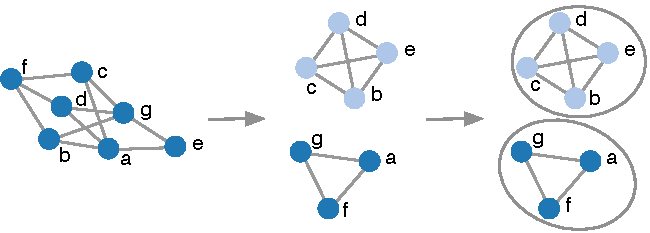
\includegraphics[width=0.9\columnwidth]{figures/examples/examplegraphs.pdf}
\end{center}
\caption{Method overview. A correlation graph is transformed to a similarity graph, in which clustering is performed.}
\label{fig:examplegraphs}
\end{figure}

\begin{sloppypar}
As a simple example, consider the set of concepts $C = \{a,b,c,d,e,f,g\}$ with the symmetric, binary correlation graph shown to the left in Fig.\ \ref{fig:examplegraphs}. Each of the concepts $a$, $f$, and $g$ has a relation to $c$, $d$, $e$, and $d$.
\end{sloppypar}

Transforming this correlation graph to the similarity graph shown in the same figure using Eq.\ \ref{eq:sim}, the pairwise similarities become positive when two concepts have overlapping contexts. Each of these clusters is  identified as a higher order concept.

Note that in the case of the binary relationship graph, the $L_1$-norm between two concepts, $i$ and $j$, is given by the number of neighbours that they do not share:
\begin{equation}
\dnm{i}{j} = |n_i \cup n_j| - |n_i \cap n_j| = |n_i| + |n_j| - 2 |n_i \cap n_j|,
\label{eq:binarynorm}
\end{equation}
where $n_i$ and $n_j$ are the neighbourhoods of $i$ and $j$. Since the maximum possible norm of the difference is $|n_i| + |n_j|$, the similarity between $i$ and $j$ becomes
\begin{equation}
\sy{i,j} = 1 - \frac{|n_i| + |n_j| - 2 |n_i \cap n_j|}{|n_i| + |n_j|} = \frac{2 |n_i \cap n_j|}{|n_i| + |n_j|},
\label{eq:binaryrelnorm}
\end{equation}
which is known as the S{\o}rensen-Dice coefficient \cite{Dice45,Sorensen48}. This similarity measure is analogous to the commonly used Jaccard coefficient \cite{Chao-2005} through a monotonic transformation.

\section{Methods}
\label{sec:methods}

While we discuss methods for constructing a correlation graph in later sections, the main contribution of this paper with
regard to methods is a scalable algorithm for transforming a correlation graph into a similarity graph. The algorithm relies on
two observations that allow us to approximate the similarities in a controlled manner.

\subsection{Similarity calculations}
\label{sec:similaritycalculations}

Firstly, a concept only has a degree of similarity to its second-order neighbours (its neighbours' neighbours) in the
correlation graph $\mathcal{R}$. Let $n_i$ and $n_j$ be the neighbouring vertices of $i$ and $j$ respectively, and $\rn{i,
k} = 0$ if $k \not\in n_i$. Then
\begin{eqnarray}
\nm{i,j}  =
\sum_{k \in n_i}  |\rn{i, k}| -  \sum_{\mathclap{k \in n_i \cap n_j}}  |\rn{i, k}| \notag\\
+  \sum_{k \in n_j}  |\rn{j, k}| -  \sum_{\mathclap{k \in n_i \cap n_j}}  |\rn{j, k}|
+  \sum_{\mathclap{k \in n_i \cap n_j}} |\rn{i, k} - \rn{j, k}| \notag\\
=  \rns{i} + \rns{j} + \sum_{\mathclap{k \in n_i \cap n_j}} (|\rn{i, k} - \rn{j, k}| - |\rn{i, k}| - |\rn{j, k}|). \label{eq:l1terms}
\end{eqnarray}
When calculating Eq.\ \ref{eq:sim} it is therefore sufficient to compare differences between weights $\rn{i, k}$ and
$\rn{j, k}$ of edges from $i$ and $j$ to neighbours $k$ that $i$ and $j$ have in common, give that we have the weight
sums of outgoing edges of $i$ and $j$.

In practice we generate a similarity graph by first summing weights of outgoing edges per vertex, and then building an
intermediate undirected two-hop multigraph of $\mathcal{S}$, where an edge $(i, j)$ that correspond to a hop through
$k$ in $\mathcal{S}$ has weight $|\rn{i, k} - \rn{j, k}| - |\rn{i, k}| - |\rn{j, k}|$. The $L_1$-norm between $i$ and
$j$ is then calculated by summing the weights of all edges between $i$ and $j$ in the multigraph according to Eq.\
\ref{eq:l1terms}, and adding this to the edge weight sums of $i$ and $j$.

\subsubsection{Approximations}
\label{subsec:approximations}
Even though we only need to consider shared neighbors when calculating the similarities between concepts, these
calculations still scale unfavorably as the sum of the square of in-degrees per vertex, since we consider all pairs of
incoming edges of vertex $k$ when generating two-hop edges. We therefore need to approximate the similarity measure by
reducing in-degrees. To be able to determine whether a certain concept distance with regard to a distance measure $D$ is
relevant or not, typically we would like to ensure that the error $E_{D}(i,j)$ in any specific distance approximation
is less than a fixed level $\theta_D$,
\begin{equation}
E_{D}(i,j) \leq \theta_D
\end{equation}
and more specifically for the $L_1$-norm approximated by $\tilde{L}_1$,
\begin{equation}
E_1(i,j) = | \nm{i,j}  - \anm{i,j}  | \leq \theta_1.
\end{equation}

%Note that the expected value of $E_{D}(i,j)$ increases as the number of concepts $|C|$ in the calculation increases. Thus, it might be easier to specify the precision of the calculations using the mean correlation error
%\begin{equation}
%E_\xi = \frac{E_{D}(i,j)}{|C|} \leq \theta_\xi
%\end{equation}

%\subsubsection{Removing low-correlation terms}
%\label{sec:removinglowcorr}

To do similarity calculations for all pairs of concepts at scale, effectively we need to reduce the number of terms in Eq.\ \ref{eq:l1terms}. First, let us note that
\begin{equation}
\label{eq:corrapprox}
| \rn{i,k} - \rn{j,k} | \approx \rn{i,k}, \quad \rn{i,k} \gg \rn{j,k}
\end{equation}
and that the error we make in the approximation is
\begin{equation}
\label{eq:corrapproxbound}
\varepsilon_k(i, j) = | \rn{i,k} - (| \rn{i,k} - \rn{j,k} | ) | \leq \rn{i,k}, \rn{j,k}
\end{equation}
Thus, if we would like to remove terms in the calculation by approximating by zero while keeping the total approximation error $E_D$ as small as possible, we should remove the smallest relation terms $\rn{i,k}$ in Eq.\ \ref{eq:l1terms}.

%\subsection{Error bound}
Let $\mrn{i}$ be a threshold value below which relations of concept $i$ are approximated by zero, and $\drns{i}$ be the norm of discarded relations:
\begin{equation} \label{}
\drns{i} = \sum_{ \rn{i,k} < \mrn{i}} |\rn{i,k}|.
\end{equation}
The upper bound of the error is then given by
\begin{equation} \label{eq:errbound}
E_1(i,j) \leq \drns{i} + \drns{j},
\end{equation}
where $E_1(i,j)=\drns{i} + \drns{j}$ when the edges of discarded relations of $i$ and $j$ do not share any destination
vertex $k$. When calculating the concept similarity based on the $L_1$-norm, we can therefore reduce the number of
terms we need to compare by removing low relation values with predictable errors. Lowering the number of terms in
Eq.\ \ref{eq:l1terms} while guaranteeing an error $E_1(i,j) \leq \theta_1$ is then a matter of sorting correlations
$\rn{i,k}$ and, starting with the smallest one, removing all relations until the cumulative sum exceeds half the
distance error threshold, $\theta_1/2$.

This brings us to our second observation, which is that in most realistic large correlation graphs, a substantial fraction of
the correlations from one concept to others are, if not zero, very small or even magnitudes smaller than its largest
relations, as exemplified in Fig.\ \ref{fig:billion-ew-cdf}. Thus, we may effectively prune a
large fraction of the links while keeping the cumulative discarded weight (and error) comparatively low, reducing
computational complexity.

Moreover, if reducing terms in Eq.\ \ref{eq:l1terms} has priority over accuracy, we may start at the other end by specifying a maximum in-degree
per vertex, and keep the corresponding number of incoming edges with the largest weights. Doing so we utilize that, in
typical correlation graphs of interest, the main bulk of vertices have low in-degrees and are therefore not affected by the
pruning. This situation is for example illustrated in Fig.\ \ref{fig:billion-id-cdf}. By calculating and storing
the sums of discarded weights of outgoing edges per vertex, we can then readily calculate the error bound per concept
pair according to Eq.\ \ref{eq:errbound}.

\begin{figure}
\begin{centering}
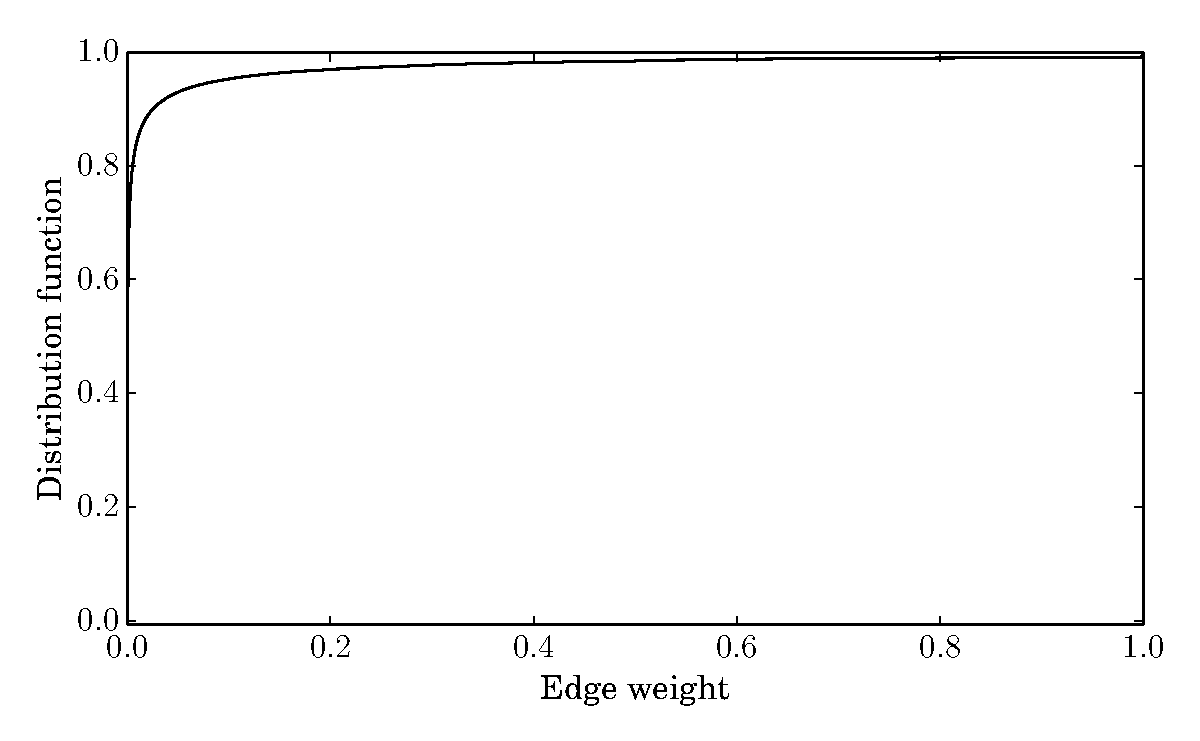
\includegraphics[width=1.0\columnwidth]{figures/billion-words/billion-ew-cdf.pdf}
\end{centering}
\caption{The cumulative distribution function of edge weights in the Billion word correlation graph described in Sec.\ \ref{subsec:words} shows that a large fraction of edges with low weights can be pruned.}
\label{fig:billion-ew-cdf}
\end{figure}

\begin{figure}
\begin{centering}
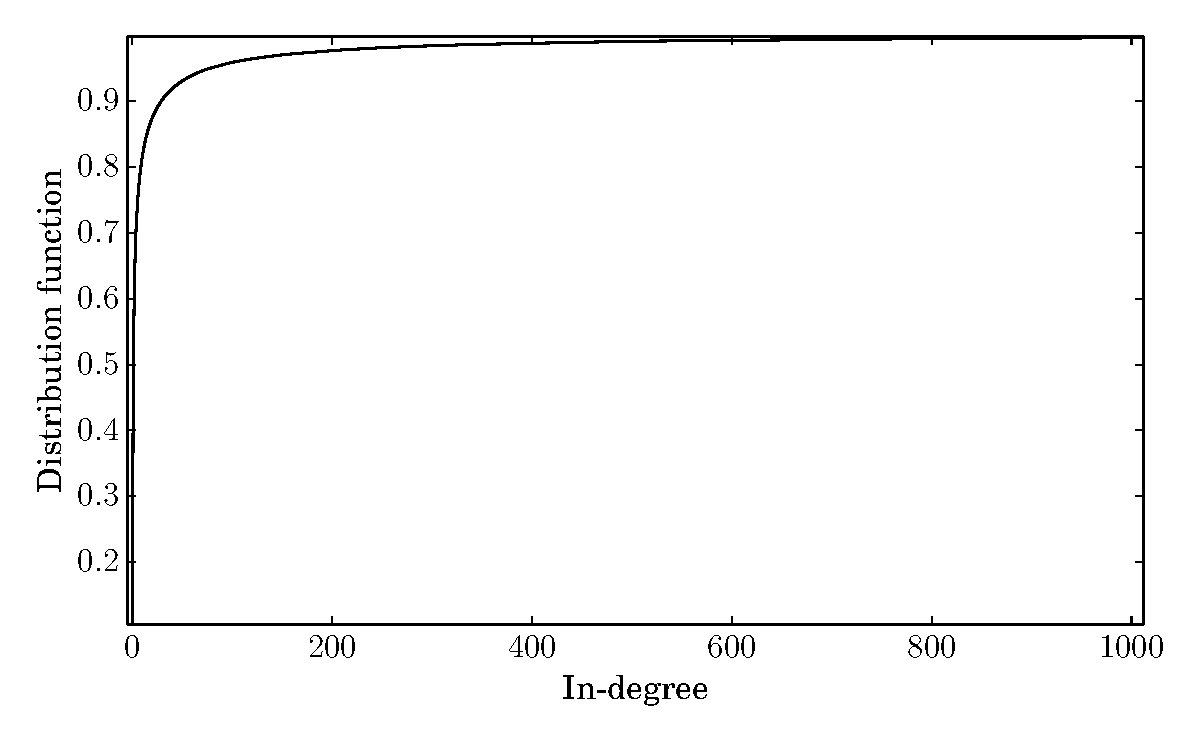
\includegraphics[width=1.0\columnwidth]{figures/billion-words/billion-id-cdf.pdf}
\end{centering}
\caption{The cumulative distribution function of in-degrees for the graph referred to in Fig.\ \ref{fig:billion-ew-cdf} illustrates that it is possible to apply an in-degree threshold while affecting comparably few vertices.}
\label{fig:billion-id-cdf}
\end{figure}

%If we instead use a mean correlation error limit $\theta_\xi$, this is as simple as removing all correlations $\rn{i,k} \leq \theta^\xi$. Note though that in any implementation where edges from $i$ are approximated as zero, it is important to calculate the error based on $\rn{i,k}$ and not $\rn{j,k}$ as this will lead to a tighter bound on the error (see equation \ref{eq:corrapproxbound}).

\subsection{Clustering}
\begin{sloppypar}
After transforming a correlation graph to a similarity graph, the latter typically exhibits tightly grouped
concepts that are similar according to measure $\sy{i,j}$. We can therefore identify higher-order concepts by
clustering the vertices, which is also known as community detection. There is an abundance of available algorithms
(see \cite{Fortunato-2010} for a review) with varying suitability with regard to accuracy and scalability. However, it is
beyond the scope of this paper to evaluate the performance of different clustering algorithms in this context.
For this reason, and in order to facilitate
our understanding for the properties of the method outlined in \ref{sec:similaritycalculations},
we choose to use a simple and transparent clustering method. The approach resembles standard distributed algorithms
for identifying connected components in graphs and works as follows: We begin by initializing
each vertex $i$ to form its own cluster, indexed by $c_i = i$. Then, for each vertex $i$, we set its cluster index to be the smallest cluster
index of $i$:s neighbours $j$ for which $\sy{i,j} \geq \sigma_{min}$, where $\sigma_{min}$ is a threshold value. This is repeated until no more cluster indices are changed. In this way, cluster memberships are propagated within
components that are separated by edges with weights $\sy{i,j} \leq  \sigma_{min}$. The interpretation of --
and rationale for -- this approach is that clusters in the graph are groups of vertices that are interlinked with a certain degree of similarity,
as specified by $\sigma_{min}$, and where the clusters, in turn, are interlinked with weaker similarity relations.
\end{sloppypar}

\subsection{Algorithms and implementation}
\label{subsec:algorithmsAndImplementation}

\begin{figure*}
\begin{lstlisting}
1: ins   = edges.map(((i,j),rij) => (j,(i,rij)))
2: pairs = ins.join(ins).filter((k,((i,rik),(j,rjk))) => i < j)
3: terms = pairs.map((k,((i,rik),(j,rjk))) => ((i,j),abs(rik-rjk)-abs(rik)-abs(rjk)))
4:              .reducebykey((v, w) => v + w)
\end{lstlisting}
\caption{Pseudo-code of sum term calculation in Eq.\ \ref{eq:l1terms}. 1) Edge tuples with vertex indices \texttt{i} and \texttt{j}, and weights \texttt{rij} are mapped to key-value pairs keyed by destination vertices. 2) A two-hop graph is generated through self-join, and unique in-edge pairs are extracted through filtering. 3) All terms in the sum in Eq.\ \ref{eq:l1terms} are calculated and 4) summed per two-hop neighbour pair.
}
\label{fig:pseudocode}
\end{figure*}

The calculations of the approximations and error bounds of the norms of the differences
$\dnm{i}{j}$, as formulated in Eq. \ref{eq:l1terms}, lend themselves well to functional
programming, since they can be implemented as a small number of standard transformations applied
on a list of correlation graph edges. The procedure can be summarized in the following
steps:
\begin{enumerate}
\item Prune the correlation graph by filtering out edges with weights below a given threshold value, $\mrn{i}$, and/or by keeping a given number of incoming edges with the largest weights per vertex.
\item For each vertex $i$, calculate the norms $\rns{i}$ (the weight sum prior
to pruning), $\drns{i}$ (the weight sum of discarded edges) and $\krns{i}$
(the weight sum of kept edges), where $\drns{i}$ is simply acquired by
subtracting $\krns{i}$ from $\rns{i}$.
\item Calculate the sum term in Eq.\ \ref{eq:l1terms}, denoted $\Lambda_{i,j}$,
for each pair of vertices that share a neighbour in the pruned correlation graph.
This step is described in pseudo-code in Fig.\ \ref{fig:pseudocode} and
involves a self-join operation for building a two-hop multigraph that links
second-order neighbours, followed by a map transformation for calculating the
terms in the sum, which subsequently are summed up per vertex pair by a reduce
operation.
\item For each vertex pair $(i,j)$ in the previous step, calculate the
approximate relative $L_1$-norm, $\tilde{l}_{i,j}$, as $\tilde{l}_{i,j} =
(\Lambda_{i,j} + \psi_{i,j})/\psi_{i,j}$ and the upper error bound,
$\epsilon_{i,j}$, as $\epsilon_{i,j} = (\drns{i} + \drns{j})/\psi_{i,j}$,
where the normalizing factor $\psi_{i,j} = \rns{i} + \rns{j}$ is
the maximum possible difference between $i$ and $j$.
\end{enumerate}
After completing step 4 it is straightforward to calculate the approximate
similarity $\asy{i,j} = 1 - \tilde{l}_{i,j}$ according to Eq.\ \ref{eq:sim}.
Note that $\tilde{l}_{i,j}$ is a conservative approximation of the true
relative $L_1$-norm, $l_{i,j}$, since $\tilde{l}_{i,j} - \epsilon_{i,j} \leq
l_{i,j} \leq \tilde{l}_{i,j}$. For this reason, the acquired similarity
approximation will be the ``worst case scenario'' in the sense that it is always larger than the true relative $L_1$-norm.

The method is implemented in the Scala programming language and uses the in-memory
data processing framework Spark \cite{Zaharia-2012}, which enables us
to employ the method at scale in terms of computing hardware.
To facilitate reproducibility, the implementation will be made available
with an open source license in an online repository\footnote{https://github.com/sics-dna/concepts}.
Since we are exclusively using standard core primitives in Spark (\texttt{map},
\texttt{filter}, \texttt{join} etc.), implementing the
method in other similar frameworks, such as Flink \cite{Alexandrov14}, is also
possible.

\section{Experiments}

\subsection{Words}
\label{subsec:words}

\begin{figure*}
\begin{center}
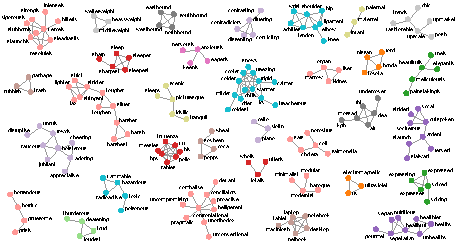
\includegraphics[width=0.9\textwidth]{figures/examples/billion-words-example.pdf}
\end{center}
\caption{Higher-order concepts in a word similarity graph based on the Billion word corpus are constituted by clusters of similar words. For sake of clarity, edges with weights $\sy{i,j} \geq 0.15$ are shown.}
\label{fig:billion-words-example}
\end{figure*}

We begin by relating words in terms of their co-occurrence in text, where two words, $i$ and $j$, co-occur if they both
appear within a window of $n$ words. In the simplest case, for $n = 2$, words therefore co-occur if they are adjacent.
There exists many different word association measures, see \cite{Pecina08} for a large number of examples, such as
pointwise mutual information \cite{Church90} and normalized versions thereof \cite{Bouma09}. Here we simply measure the
association between $i$ and $j$ as the relative frequency of $j$ occurring in $i$:s context, or, in other words, as the
conditional probability that a randomly selected word in a window that contains $i$, will be the word $j$. That is, $\rn{i,j}
\approx c_{i,j}/{c_i}$, where $c_i$ and $c_{i,j}$ are the number of occurrences of $i$, and $i$ together with $j$,
respectively. Note that this measure is not symmetric and so $\rn{i,j} \neq \rn{j,i}$ may be true. There likely exists more
appropriate measures, such as pointwise mutual information mentioned above, with regard to specific applications.
However, for the purpose of demonstrating the proposed method, we believe the conditional probability measure suffices.

The method is applied on two datasets: the Billion word \cite{Chelba13} and
the Google Books n-gram \cite{Michel10,Lin12} corpora. The former consists of
nearly one billion words and originates from crawled online news texts. From
these we count the number of occurrences of bigrams, pairs of adjacent words, with words consisting only
of alphabetic characters. This results in approximately 8 million unique
bigrams and a vocabulary with roughly 0.3 million words. From the bigram counts
we relate words by their ordered adjacency, where the co-occurrence window of a focus word
is the set of subsequent words.

Despite the comparably modest size of this corpus, the method
manages to discover groups of words that reflect both syntactic and semantic
concepts. Examples of such higher-order concepts are shown in Fig.\ \ref{fig:billion-words-example},
where we see that the clusters e.g. correspond to specific nouns,
 (\emph{tablet}, \emph{laptop}, \emph{notebook} etc.), adjectives
 (\emph{chic}, \emph{trendy}, \emph{fashionable} etc.), or adverbs
 (\emph{strongly}, \emph{intensely}, \emph{vigorously}, etc.).

\begin{sloppypar}
The Google Books n-gram dataset, which consists of 361
billion tokens for the English language version of the dataset, is used both to evaluate the scalability of the
method, which will be discussed in Sec.\ \ref{sec: scalability}, and to quantify the quality of resulting similarity
relations. An n-gram can be defined as a contiguous sequence of $n$ words in a text.
To further challenge the method, we apply it on correlation graphs with respect to co-occurrence
windows of size 5. This results in a denser correlation graph, since a
word has more neighbors due to the larger co-occurrence window size. Nevertheless, the
key properties that we describe in Sec.\ \ref{subsec:approximations} still
apply and we can prune away a large number of edges with low weights.
\end{sloppypar}

A common approach to evaluate the performance of word association methods is to use benchmarks
with word pairs that have been manually graded with respect to degree of association. Since these
benchmarks also contain unassociated words, it is not possible to do a direct comparison between our
method and other
approaches in terms of benchmark performance, since our method only relates words that have a certain
degree of similarity (indeed, this is one of the reasons it is scalable). However, to give an indication of
the method's performance, we measure the Spearman rank correlation coefficient between benchmark
similarities and $\sy{i,j}$ for word pairs $(i, j)$ that \emph{do} exist in the similarity graph. For this purpose we
use the standard WS-353 test collection \cite{Finkelstein01}, which consists of 353 word pairs that have
been graded by human annotators. We build a similarity graph from co-occurrence windows of size 5, filter
out words that occur with a frequency less than $10^{-8}$ and edges $\rn{i,j} < 10^{-3}$, and
sets the maximum in-degree to 200. In this graph, which is built in less than 10 minutes (cf. Fig.\ \ref{fig:google-e-runtime}),
60\% of the WS-353 word pairs are present, resulting in a Spearman rank correlation of 0.76. The current state of the
art (with respect to the whole dataset) is 0.81 \cite{Halawi12,Yih12}.
These figures represent the correlation with respect to the average annotator score. Note though
that there is low inter-annotator agreement in WS-353. The mean performance
of individual annotators, with respect to the mean score of the remaining annotators, is also 0.76 \cite{Hill14}.

\subsection{Artists}
In the next proof of concept we relate artists by using a dataset that represents the listening
habits of users of the \emph{Last.fm} music service.\footnote{http://www.last.fm/} This dataset, provided by Celma
\cite{Celma2010}, consists of approximately 19 million track plays of 992 users. For each user, we extract sequences of
played artists - there are roughly 177000 in total - and consider the context of an artist to be defined by the probability
distribution of subsequently played artists. Hence, we assume artists are related in a Markov chain, where each artist
constitutes a state, and where there is a directed edge from artist $i$ to artist $j$ weighted with the probability
that $j$ is played next, given that $i$ is currently playing. This probability is simply estimated as $\rn{i,j} \approx
c_{i,j}/c_i$, where $c_i$ and $c_{i,j}$ are the number of times $i$, and $i$ followed by $j$ occur in the data set,
respectively.

The in-degree distribution of the artist correlation graph resembles those of the word correlation graphs,
which again means that relatively few vertices are affected by in-degree pruning. Transforming the artist correlation
graph to a similarity graph also results in tightly grouped artists that can be clustered. The resulting
clusters appear to represent musical genres as exemplified in Fig.\ \ref{fig:artists}. These clusters can in turn be grouped
into higher order groups, and so the similarity graph can be interpreted as a map over music genres and sub-genres.

As such, the output of this task could be used in a music recommendation system providing relations between artists that
are generated by the listening habits of users, similar to a collaborative filtering system. This makes the system differ
from the co-occurrence based artist similarity measure presented in \cite{schedl2005web}, where the authors define
artist-to-artist similarity based on the number of online search engine results, as was the approach
in \cite{Cilibrasi-2007}. Moreover, our system could provide an intuitive way to incorporate the popularity of artists through
their play frequencies, and in extension to mitigate the effect of popularity bias in recommendations \cite{celma2008hits}.

\begin{figure}
\begin{centering}
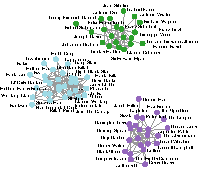
\includegraphics[width=0.95\columnwidth]{figures/examples/last-fm-example-3.pdf}
\end{centering}
\caption{Examples of clusters in an artist similarity graph correspond to thee distinct music genres. Edges with weights $\sy{i,j} \geq 0.5$ are shown.}
\label{fig:artists}
\end{figure}

\subsection{Codons}

To further demonstrate the broad applicability of our approach, we finally apply the method in the field of molecular biology.
Here we consider codons as first order concepts. Codons are triplets of
adjacent nucleotides in DNA, that translate to amino acid residues that in turn form proteins.  These are related
through codon substitution dynamics, which is central both for understanding molecular evolution and in applications
such as DNA sequence alignment \cite{Anisimova09}. Since there are only 64 codons in total, this example differs from
the previous two in that we consider relatively few concepts.

Codon substitutions are often modeled as Markov processes (see \cite{Anisimova09} for an extensive review), where the
substitution probabilities of a codon at a specific location are assumed to be independent of neighbouring codons as
well as previous codons at the same location.

In this example we use an empirically derived codon substitution matrix provided by Schneider et al.
\cite{Schneider2005}, where we consider the context of a codon $i$ to be given by the relative substitution frequencies
$(\rn{i,j})_{j=1}^n$ to other codons $j$.

\begin{figure}
\begin{centering}
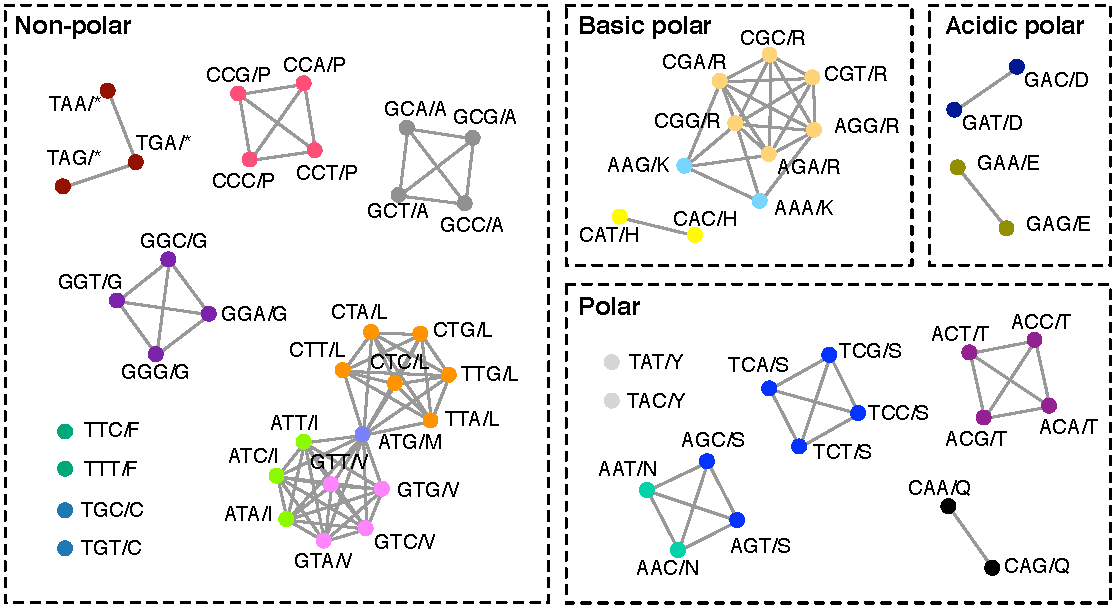
\includegraphics[width=1.0\columnwidth]{figures/examples/codon-example.pdf}
\end{centering}
\caption{Codon similarity graph where vertices are labeled with $c/a$ for codon $c$ coding to amino acid $a$. Edges
with weights $\sy{i,j} \geq 0.45$ are shown. Vertices are color coded with respect to amino acids and grouped by
properties. Note that when the edge weight threshold is lowered, clusters containing several amino acids are split by
amino acid. The rare and low mutable amino acid tryptophan is omitted. }
\label{fig:codons}
\end{figure}

As seen in the resulting codon similarity graph in Fig.\ \ref{fig:codons}, codons that translate to the same amino acid according
to the standard genetic code \cite{Nirenberg65} tend to be grouped. This reflects that codons that are highly similar
literary are commutable since substitutions between these codons are neutral under evolution. These clusters are also
present in the correlation graph and therefore preserved through the similarity graph transformation.

We now shift perspective and view ``amino acid'' as a higher-order concept. Again looking at Fig.\ \ref{fig:codons},
we see that some of the amino acids are grouped. This can be explained by a higher degree of neutrality within groups
than between them, which has been observed in empirical amino acid substitution matrices, such as the accepted point
mutation (PAM) matrix by Dayhoff et al. \cite{Dayhoff78}. In comparison, Wu and Brutlag derived amino acid substitution
groups by group-wise (as opposed to pairwise) statistical analysis of protein databases \cite{Wu96}.  The groups shown
in Fig.\ \ref{fig:codons} (\{I, L, M, V\}, \{K, R\} and \{N, S\}) all agree with their findings.

\begin{sloppypar}
In summary, the codon similarity graph captures two higher-order concepts: From codons to amino acids, via the genetic code, to higher-order amino acids that constitute known substitution groups.
\end{sloppypar}

\section{Scalability}
\label{sec: scalability}

In order to enable practical use of the algorithms on large tasks in terms of the number of concepts, correlations and example data,
a key design goal is scalability. Since we are using
relational primitives to represent graphs,
the scalability of the algorithm can be studied using established results from
relational algebra \cite{Chandra77, bitton83}. The most computationally demanding component of the algorithm is
building the two-hop graph through a self-join operation (the third step in Sec.\ \ref{subsec:algorithmsAndImplementation}).

%which is the calculation of the sum term in\ \ref{eq:l1terms}. This operation is a potential bottleneck in the
%algorithm \comment{or should we say the most computationally costly step?}
%as it requires a self-join of the edges table, which can contain millions of rows.

\begin{figure}
\begin{centering}
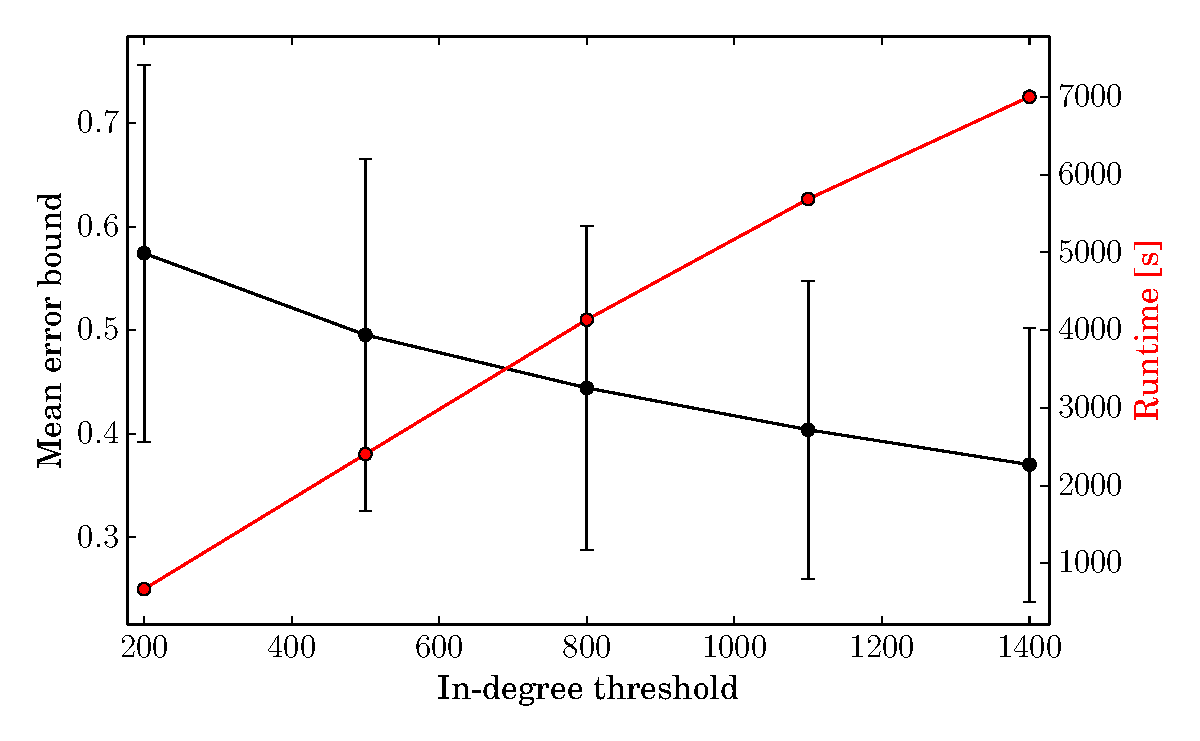
\includegraphics[width=1.0\columnwidth]{figures/billion-words/billion-e-rt-2.pdf}
\end{centering}
\caption{Runtime, mean error bound and standard deviation of error bound (shown as error bars) for different in-degree thresholds, and $\rn{i,j} \geq 10^{-5}$. Built from bigrams in the Billion word corpus using a standard commodity laptop.}
\label{fig:billion-e-runtime}
\end{figure}

Since a self-join is a conjunctive query \cite{Chandra77} in relational algebra terms,
we can reason about its computational cost.
Specifically for a distributed environment, Koutris et al. \cite{koutris2011conjuctive}
define a parallel algorithm as a sequence of parallel computation steps, and define its
cost as the number of steps required to complete the algorithm.
The authors prove that a join operation can be completed in one parallel computational
step using the hash-join algorithm, by using a communication and a computation phase.
Just as importantly they prove that the hash-join operation is load balanced
and as such it ensures linear speedup (doubling the server count reduces the load by
half) and constant scaleup (when doubling both the size of the data and number of servers, the running time remains the same).
%In the case of the self-join one could also avoid the communication step and apply
%the join operation on the parts of the distributed table that are available
%locally at each node. This would further reduce the computational requirements of the
%algorithm.

Specifically for the Spark platform, on which we implement the algorithm,
the self-join operation creates what Zaharia et al.\ \cite{Zaharia-2012}
call a \textit{narrow dependency}. This property allows for pipelined executions
of all operations on one node up until the reduction step in Fig. \ref{fig:pseudocode}, without the need for expensive data shuffles
through the network.

To demonstrate that our approach is applicable at scale in practice, we apply it on one of the largest, to our knowledge,
text corpora currently available, the Google Books
n-gram dataset \cite{Michel10,Lin12}, which corresponds to approximately 4\% of all books ever printed.
The dataset is publicly available, and in our experiments we use
the version that is available through the Amazon S3 service\footnote{https://aws.amazon.com/datasets/8172056142375670}
As described in Sec.\ \ref{subsec:words}, we use the English language corpus
which contains approximately 361 billion tokens. When processed into 5-grams, the corpus results in a file with 24.5 billion rows and the total compressed size of the dataset
is 221.5 GB. This data is pre-processed to create the correlation graph by retaining
only alphabetic characters. The resulting correlation graph before pruning has 706,108 vertices and 94,945,991 edges.

To perform the experiments we employ an Apache Spark cluster created using the Amazon
Web Services EC2 service\footnote{http://aws.amazon.com/ec2/}.
The cluster consists of 8 nodes (1 master and 7 slaves), where each node has 4 vCPUs and
30.5 GiB of memory (EC2 instance type r3.xlarge), such that the total amount of memory available to the cluster
is roughly 186 GiB, as reported by Spark.

\begin{figure}
\begin{centering}
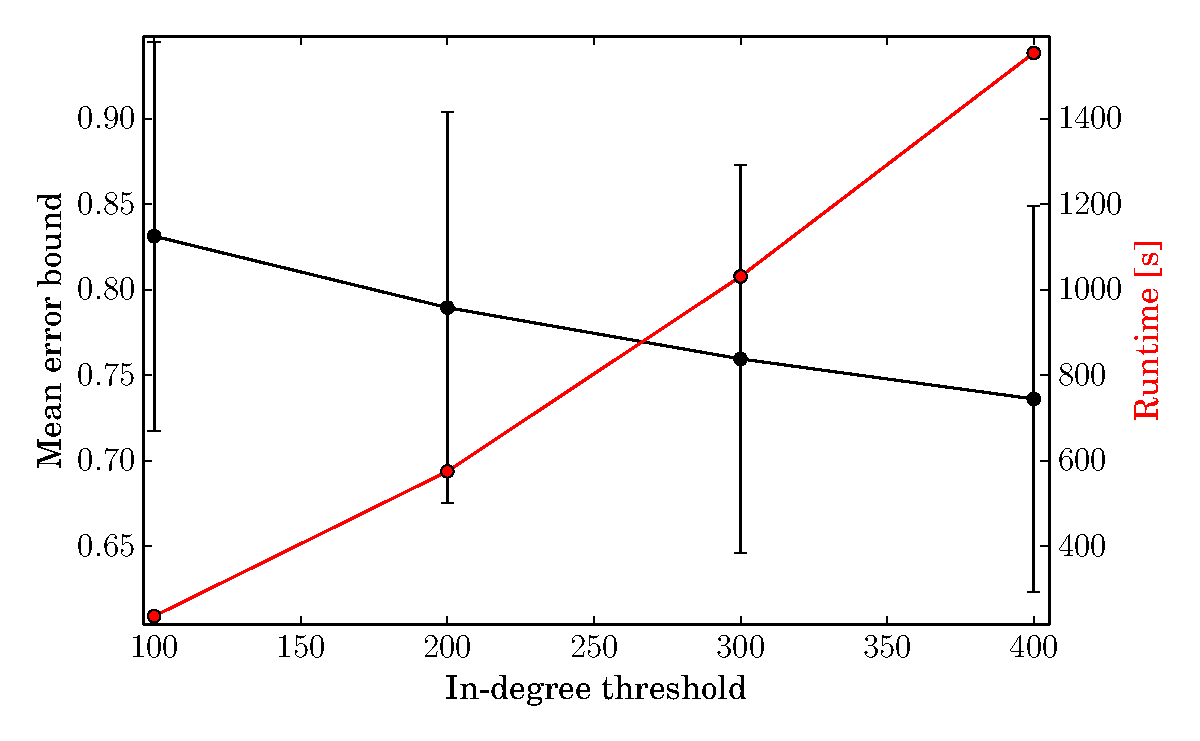
\includegraphics[width=1.0\columnwidth]{figures/google-books/eng-all-edge-low-e3-vtx-low-e8-high-e1-100-400.pdf}
\end{centering}
\caption{Runtime, mean error bound and standard deviation of error bound (shown as error bars) for different in-degree thresholds, and $\rn{i,j} \geq 10^{-3}$. Built from Google Books 5-grams using an Amazon
EC2 cluster (see text for details).}
\label{fig:google-e-runtime}
\end{figure}

The experiment results support the theoretical investigation of the computational
cost of the algorithm, and together with the pruning
described in Section \ref{subsec:approximations} we are able to transform correlation graphs into similarity
graphs in reasonable amounts of time. This also holds true when using more modest computational resources,
as shown in Fig.\ \ref{fig:billion-e-runtime}, for building similarity graphs using the Billion word corpus as described
in Sec.\ \ref{subsec:words}. Analogous results are achieved in the Google 5-gram case, here with runtimes on the order of minutes,
as seen in Fig.\ \ref{fig:google-e-runtime}. The experiments were replicated three times, and
the runtimes are reported in Table \ref{tab:google_runtimes}.
Fig.\ \ref{fig:billion-e-runtime} and Fig.\ \ref{fig:google-e-runtime} also illustrate the trade-off between accuracy, controlled
via the in-degree threshold, and runtime, where the runtime scales favourably with an increasing in-degree threshold.
With respect to the in-degree threshold, we also observe a sublinear scaling of the number of edges in the correlation
graph, and a linear growth of the number of  edges in the similarity graph,  as shown in Fig.\ \ref{fig:google-ne}. This reflects the
situation exemplified in Fig.\ \ref{fig:billion-id-cdf}, namely that comparably few vertices are affected by the in-degree threshold.

\begin{figure}
\begin{centering}
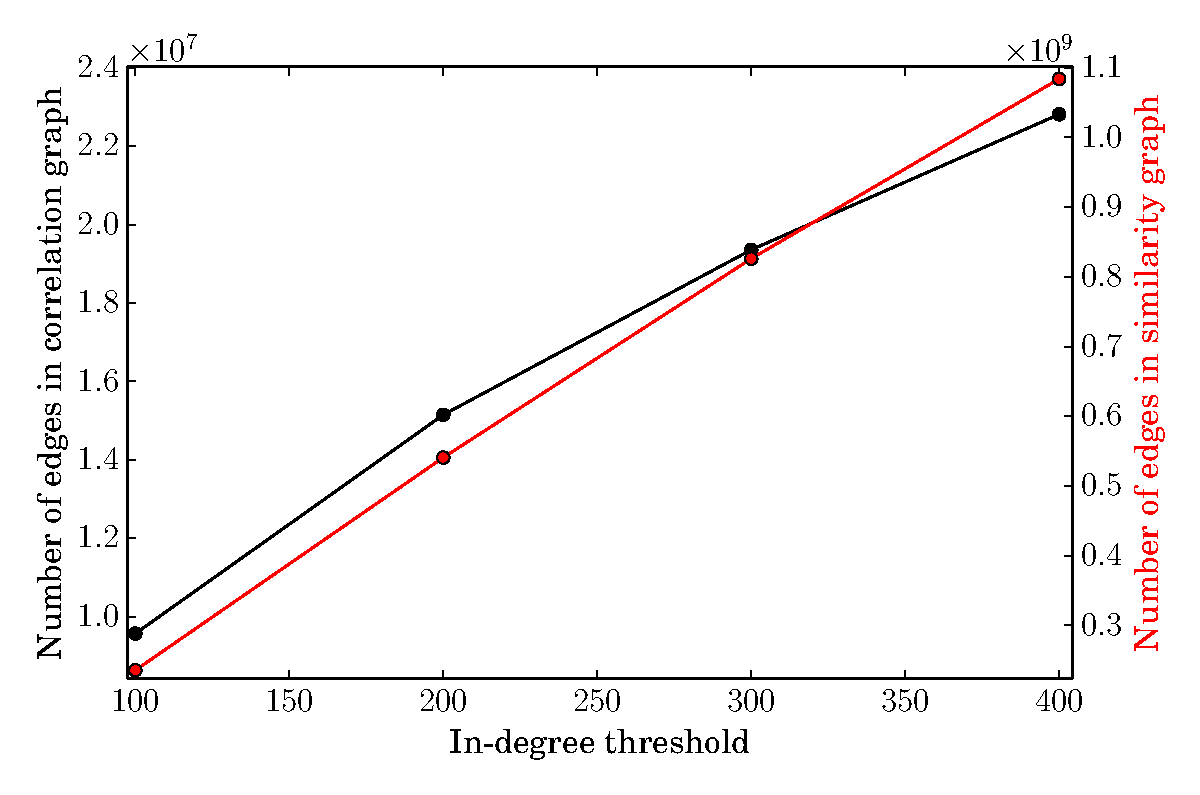
\includegraphics[width=0.95\columnwidth]{figures/google-books/eng-all-edge-low-e3-vtx-low-e8-high-e1-100-400-idg-ne-nt.pdf}
\end{centering}
\caption{Number of edges in the correlation- and similarity graph, respectively, for different in-degree thresholds. Same configuration as in Fig.\ \ref{fig:google-e-runtime}.}
\label{fig:google-ne}
\end{figure}

\begin{table}[h]
\begin{center}
\begin{tabular}{|c|r|r|r||c|c|}
  \hline In-degree  & Run 1
  & Run 2
  & Run 3
  & $\mu$
  & $\sigma$
  \\
  \hline 100
  & 246.7
  & 229.5
  & 236.7
  & 237.6
  & 8.6
  \\
  \hline 200
  & 603.7
  & 573.2
  & 575.4
  & 584.1
  & 16.9
  \\
  \hline 300
  & 1062.4
  & 998.3
  & 1031.2
  & 1030.7
  & 32.0
  \\
  \hline 400
  & 1535.5
  & 1602.5
  & 1554.0
  & 1564.0
  & 34.6
  \\
  \hline Sum & 3448.5
  & 3403.7
  & 3397.5
  & 3416.5
  & 27.7
  \\
  \hline
\end{tabular}
\end{center}
\caption{Runtimes in seconds for Google Books n-gram dataset.}
\label{tab:google_runtimes}
\end{table}

\section{Conclusions}

This paper proposes a conceptually simple method for discovering higher-order concepts trough transforming a
correlation graph to a similarity graph in which clustering is performed. As the method does not rely on any
intermediate representation or dimensionality reduction, it is applicable with few restrictions
to any domain in which a correlation graph can be constructed. Our experiments show that the approach not only can
detect relevant higher-order concepts in several types of data, but is also computationally feasible for large-scale
applications with very large number of objects.

The main methodological challenge for future work revolves around how to efficiently build hierarchical concept models.
The concepts discovered through the methods described in this paper essentially represent OR-relations: All constituent
objects of a cluster are commutable, and the higher-order concept can be said to be observed if any of its constituents
are. Analogously, strong clusters detected in the correlation graph could be considered to represent AND-relations,
where the corresponding higher-order concept is observed when all of its constituents are. Both these types of
higher-order concepts can be identified, brought back into the estimation of the correlation graph, and the process
iterated, allowing for the discovery of complex higher-order relations. How to reliably and efficiently perform this
remains an area of further study.

\newpage

\bibliographystyle{abbrv}
\bibliography{concepts-sigkdd}  % sigproc.bib is the name of the Bibliography in this case

\balancecolumns
\appendix
%\subsection{Introduction}
%Here, we outline several approximation approaches along with bounds on the errors produced.

%\subsection{Preliminaries}

%Let $C$ be a set of concepts, and $\rn{i,j}$ be a correlation (or co-occurrence) measure between concepts $i \in C$ and $j \in C$. Further, we will assume that the used correlation measure always is positive, $0 \leq \rn{i,j}$. We define the similarity between concepts $i$ and $j$ as
%\begin{equation}
%S(i, j) = \frac{1}{D(i, j)}
%\end{equation}
%where $D(i, j)$ is a distance measure between the correlation vectors of $i$ and $j$, $\Xi_{i}$ and $\Xi_{j}$ respectively. Here, we will use the $L_1$-norm which gives us the distance measure
%\begin{equation}
%\label{eq:l1div}
%D^1(i, j) = \sum_{k \in C} | \rn{i,k} - \rn{j,k} |
%\end{equation}

\section{Alternative approximations}

\subsection{Removing terms based on difference}

Implementing the similarity calculation utilizing a message passing algorithm, passing messages from $i$ to $j$
through $k$ and vice versa, removing message forwarding at $k$ could reduce the total number of messages.
The forwarding decision would in this case be dependent on the
actual difference $|\rn{i,k}-\rn{j,k}|$. However, both strategies of removing 1) high-difference messages and 2)
low-difference messages are problematic.

Removing high difference terms with bounded error, we again need to select terms where one of the relations
are small enough to approximate with zero.
Thus, combined with the approach in \ref{sec:similaritycalculations}, this is (mostly) redundant.

For the second strategy, small values of $|\rn{i,k}-\rn{j,k}|$ could be approximated as zero,
\begin{equation}
| \rn{i,k} - \rn{j,k} | \approx 0, \quad | \rn{i,k} - \rn{j,k} | \leq \theta_\varepsilon
\end{equation}
where $\theta_\varepsilon$ is a fixed relation threshold. Thus, the error by removing similar values can simply be bounded through
\begin{equation}
\varepsilon_k(i,j) = | \rn{i,k} - \rn{j,k} | \leq \theta_\varepsilon
\end{equation}
However, removing low-difference terms essentially conflicts
with the removal of low-relation terms in \ref{sec:similaritycalculations}, as we still need to send a message
indicating the approximation -- we might as well send the
actual difference.

%It is possible to use this strategy instead of the one outlined in \ref{sec:similaritycalculations}, but this would involve
%sending initial messages to all nodes, the number of which will be $|C|^2$ in total.

\subsection{Utilizing typical relation vectors}

It is in many cases reasonable to assume that the context vectors for most concepts only differ
significantly in a small number of components. We could then reduce the number of terms
in the similarity calculation by subtracting a ``typical''
context vector from all concept context vectors, and then only calculate the differences based on
components that differ significantly from zero in the resulting vectors.

Let $\rv_{\mu}$ denote the mean relation vector, calculated e.g. as
$\rv_{\mu} = \sum_{i \in C} \rv_i / |C|$,
and the difference between a relation vector $\rv_i$ and the mean relation vector $\rv_\mu$
\begin{equation}
\rv_i^{\Delta_\mu} = \rv_i - \rv_\mu , \quad  \rv_{i, j}^{\Delta_\mu} = \rn{i, j} - \rn{\mu, j}
\end{equation}
Since we are removing a constant vector from all similarity vectors, we know that
$| \rn{i,k} - \rn{j,k} | = | \rn{i, k}^{\Delta_\mu} - \rn{j, k}^{\Delta_\mu} |$,
i.e. we can calculate the distance between concepts directly in terms of the difference relation vectors. Using the $L_1$-
norm, if we remove a term $\rn{j,k}^{\Delta_\mu}$ from a similarity calculation by approximating it with zero as in section \ref{sec:similaritycalculations}, the resulting error is
\begin{equation}
\varepsilon_k(i, j) = | \rn{i,k}^{\Delta_\mu} - (| \rn{i,k}^{\Delta_\mu} - \rn{j,k}^{\Delta_\mu} | ) |
\leq | \rn{j,k}^{\Delta_\mu}|
\end{equation}
Thus, by removing terms with low-absolute value $|\rn{j,k}^{\Delta_\mu}|$ we can remove calculations and control the
error as in \ref{sec:similaritycalculations}.

\subsection{Conclusions}

We can reduce the number of terms we need to compare by removing low relations while getting predictable errors, both when working on actual relation vectors or the difference to a typical relation vector.
However, removing terms based on differences in a message passing setting is not compatible with these strategies, and
is expected to perform worse in typical cases.

\end{document}

% DOCUMENT NOTES - MOVED HERE FROM BEGINNING OF FILE
% This is "sig-alternate.tex" V2.0 May 2012
% This file should be compiled with V2.5 of "sig-alternate.cls" May 2012
%
% This example file demonstrates the use of the 'sig-alternate.cls'
% V2.5 LaTeX2e document class file. It is for those submitting
% articles to ACM Conference Proceedings WHO DO NOT WISH TO
% STRICTLY ADHERE TO THE SIGS (PUBS-BOARD-ENDORSED) STYLE.
% The 'sig-alternate.cls' file will produce a similar-looking,
% albeit, 'tighter' paper resulting in, invariably, fewer pages.
%
% ----------------------------------------------------------------------------------------------------------------
% This .tex file (and associated .cls V2.5) produces:
%       1) The Permission Statement
%       2) The Conference (location) Info information
%       3) The Copyright Line with ACM data
%       4) NO page numbers
%
% as against the acm_proc_article-sp.cls file which
% DOES NOT produce 1) thru' 3) above.
%
% Using 'sig-alternate.cls' you have control, however, from within
% the source .tex file, over both the CopyrightYear
% (defaulted to 200X) and the ACM Copyright Data
% (defaulted to X-XXXXX-XX-X/XX/XX).
% e.g.
% \CopyrightYear{2007} will cause 2007 to appear in the copyright line.
% \crdata{0-12345-67-8/90/12} will cause 0-12345-67-8/90/12 to appear in the copyright line.
%
% ---------------------------------------------------------------------------------------------------------------
% This .tex source is an example which *does* use
% the .bib file (from which the .bbl file % is produced).
% REMEMBER HOWEVER: After having produced the .bbl file,
% and prior to final submission, you *NEED* to 'insert'
% your .bbl file into your source .tex file so as to provide
% ONE 'self-contained' source file.
%
% ================= IF YOU HAVE QUESTIONS =======================
% Questions regarding the SIGS styles, SIGS policies and
% procedures, Conferences etc. should be sent to
% Adrienne Griscti (griscti@acm.org)
%
% Technical questions _only_ to
% Gerald Murray (murray@hq.acm.org)
% ===============================================================
%
% For tracking purposes - this is V2.0 - May 2012

%
% --- Author Metadata here ---
%\conferenceinfo{WOODSTOCK}{'97 El Paso, Texas USA}
%\CopyrightYear{2007} % Allows default copyright year (20XX) to be over-ridden - IF NEED BE.
%\crdata{0-12345-67-8/90/01}  % Allows default copyright data (0-89791-88-6/97/05) to be over-ridden - IF NEED BE.
% --- End of Author Metadata ---
